%%%% Better Poster latex template example v1.0 (2019/04/04)
%%%% GNU General Public License v3.0
%%%% Rafael Bailo
%%%% https://github.com/rafaelbailo/betterposter-latex-template
%%%% 
%%%% Original design from Mike Morrison
%%%% https://twitter.com/mikemorrison

\documentclass[a0paper,fleqn]{betterposter}

% For gt table latex
\usepackage{amsmath, booktabs, caption, longtable}

\usepackage{fontawesome}
% Font awesome symbols https://mirrors.ibiblio.org/CTAN/fonts/fontawesome/doc/fontawesome.pdf

%%%% Uncomment the following commands to customise the format

%% Setting the width of columns
% Left column
% \setlength{\leftbarwidth}{0.25\paperwidth}
% Right column
%\setlength{\rightbarwidth}{0.25\paperwidth}

%% Setting the column margins
% Horizontal margin
%\setlength{\columnmarginvertical}{0.05\paperheight}
% Vertical margin
%\setlength{\columnmarginhorizontal}{0.05\paperheight}
% Horizontal margin for the main column
%\setlength{\maincolumnmarginvertical}{0.15\paperheight}
% Vertical margin for the main column
%\setlength{\maincolumnmarginhorizontal}{0.15\paperheight}

%% Changing font sizes
% Text font
%\renewcommand{\fontsizestandard}{\fontsize{28}{35} \selectfont}
% Main column font
%\renewcommand{\fontsizemain}{\fontsize{28}{35} \selectfont}
% Title font
\renewcommand{\fontsizetitle}{\fontsize{72}{35} \selectfont}
% Author font
%\renewcommand{\fontsizeauthor}{\fontsize{28}{35} \selectfont}
% Section font
%\renewcommand{\fontsizesection}{\fontsize{28}{35} \selectfont}

%% Changing font sizes for a specific text segment
% Place the text inside brackets:
% {\fontsize{28}{35} \selectfont Your text goes here}

%% Changing colours
% Background of side columns
%\renewcommand{\columnbackgroundcolor}{black}
% Font of side columns
%\renewcommand{\columnfontcolor}{gray}
% Background of main column
%\renewcommand{\maincolumnbackgroundcolor}{empirical}
%\renewcommand{\maincolumnbackgroundcolor}{theory}
%\renewcommand{\maincolumnbackgroundcolor}{methods}
%\renewcommand{\maincolumnbackgroundcolor}{intervention}
% Font of main column
%\renewcommand{\maincolumnfontcolor}{gray}

\begin{document}	
\betterposter{
%%%%%%%% MAIN COLUMN

\maincolumn{
%%%% Main space

% \textbf{Urban} areas provide \textbf{habitat}
% \\to target conservation species.

% 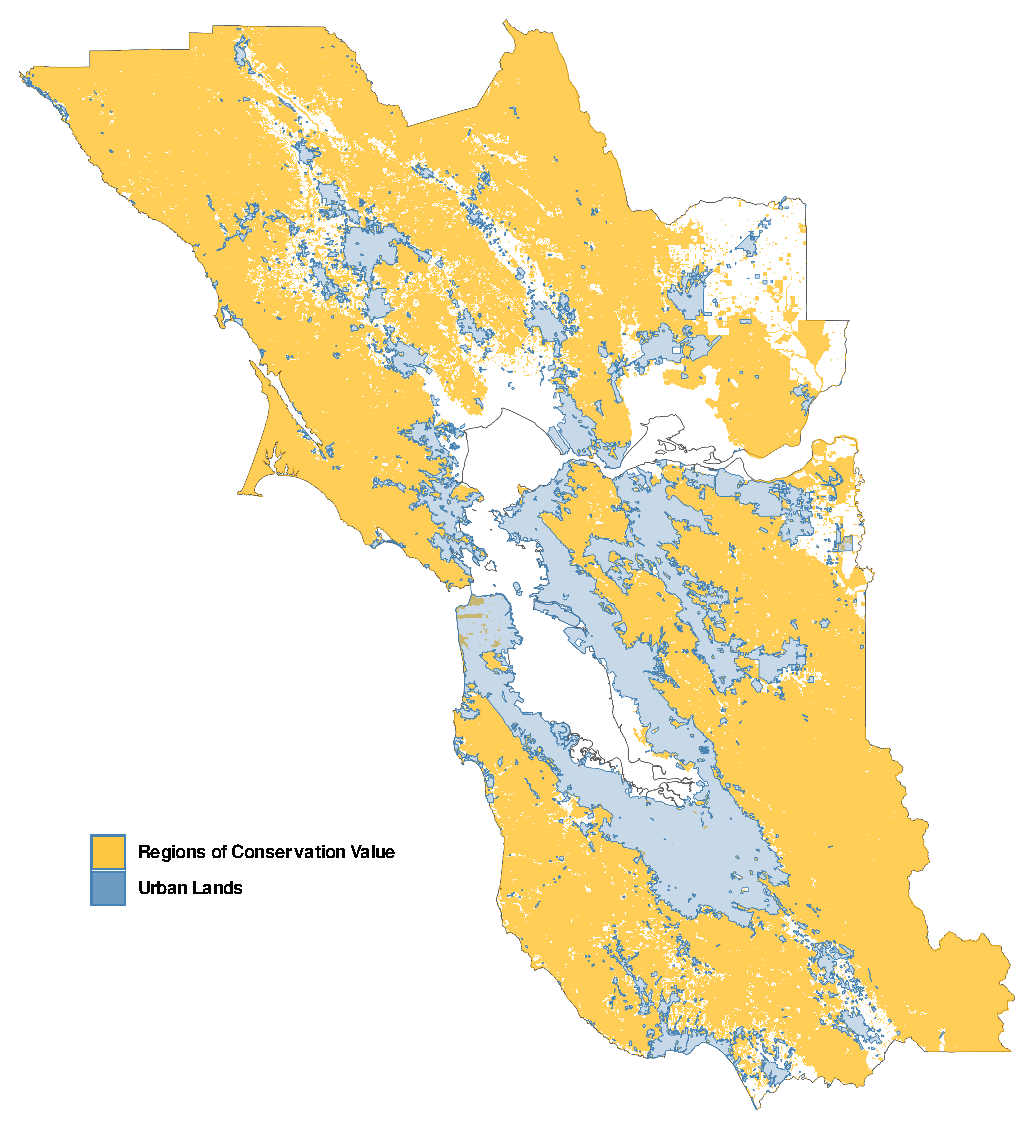
\includegraphics[width=.3\textwidth]{img/urbancln.eps}
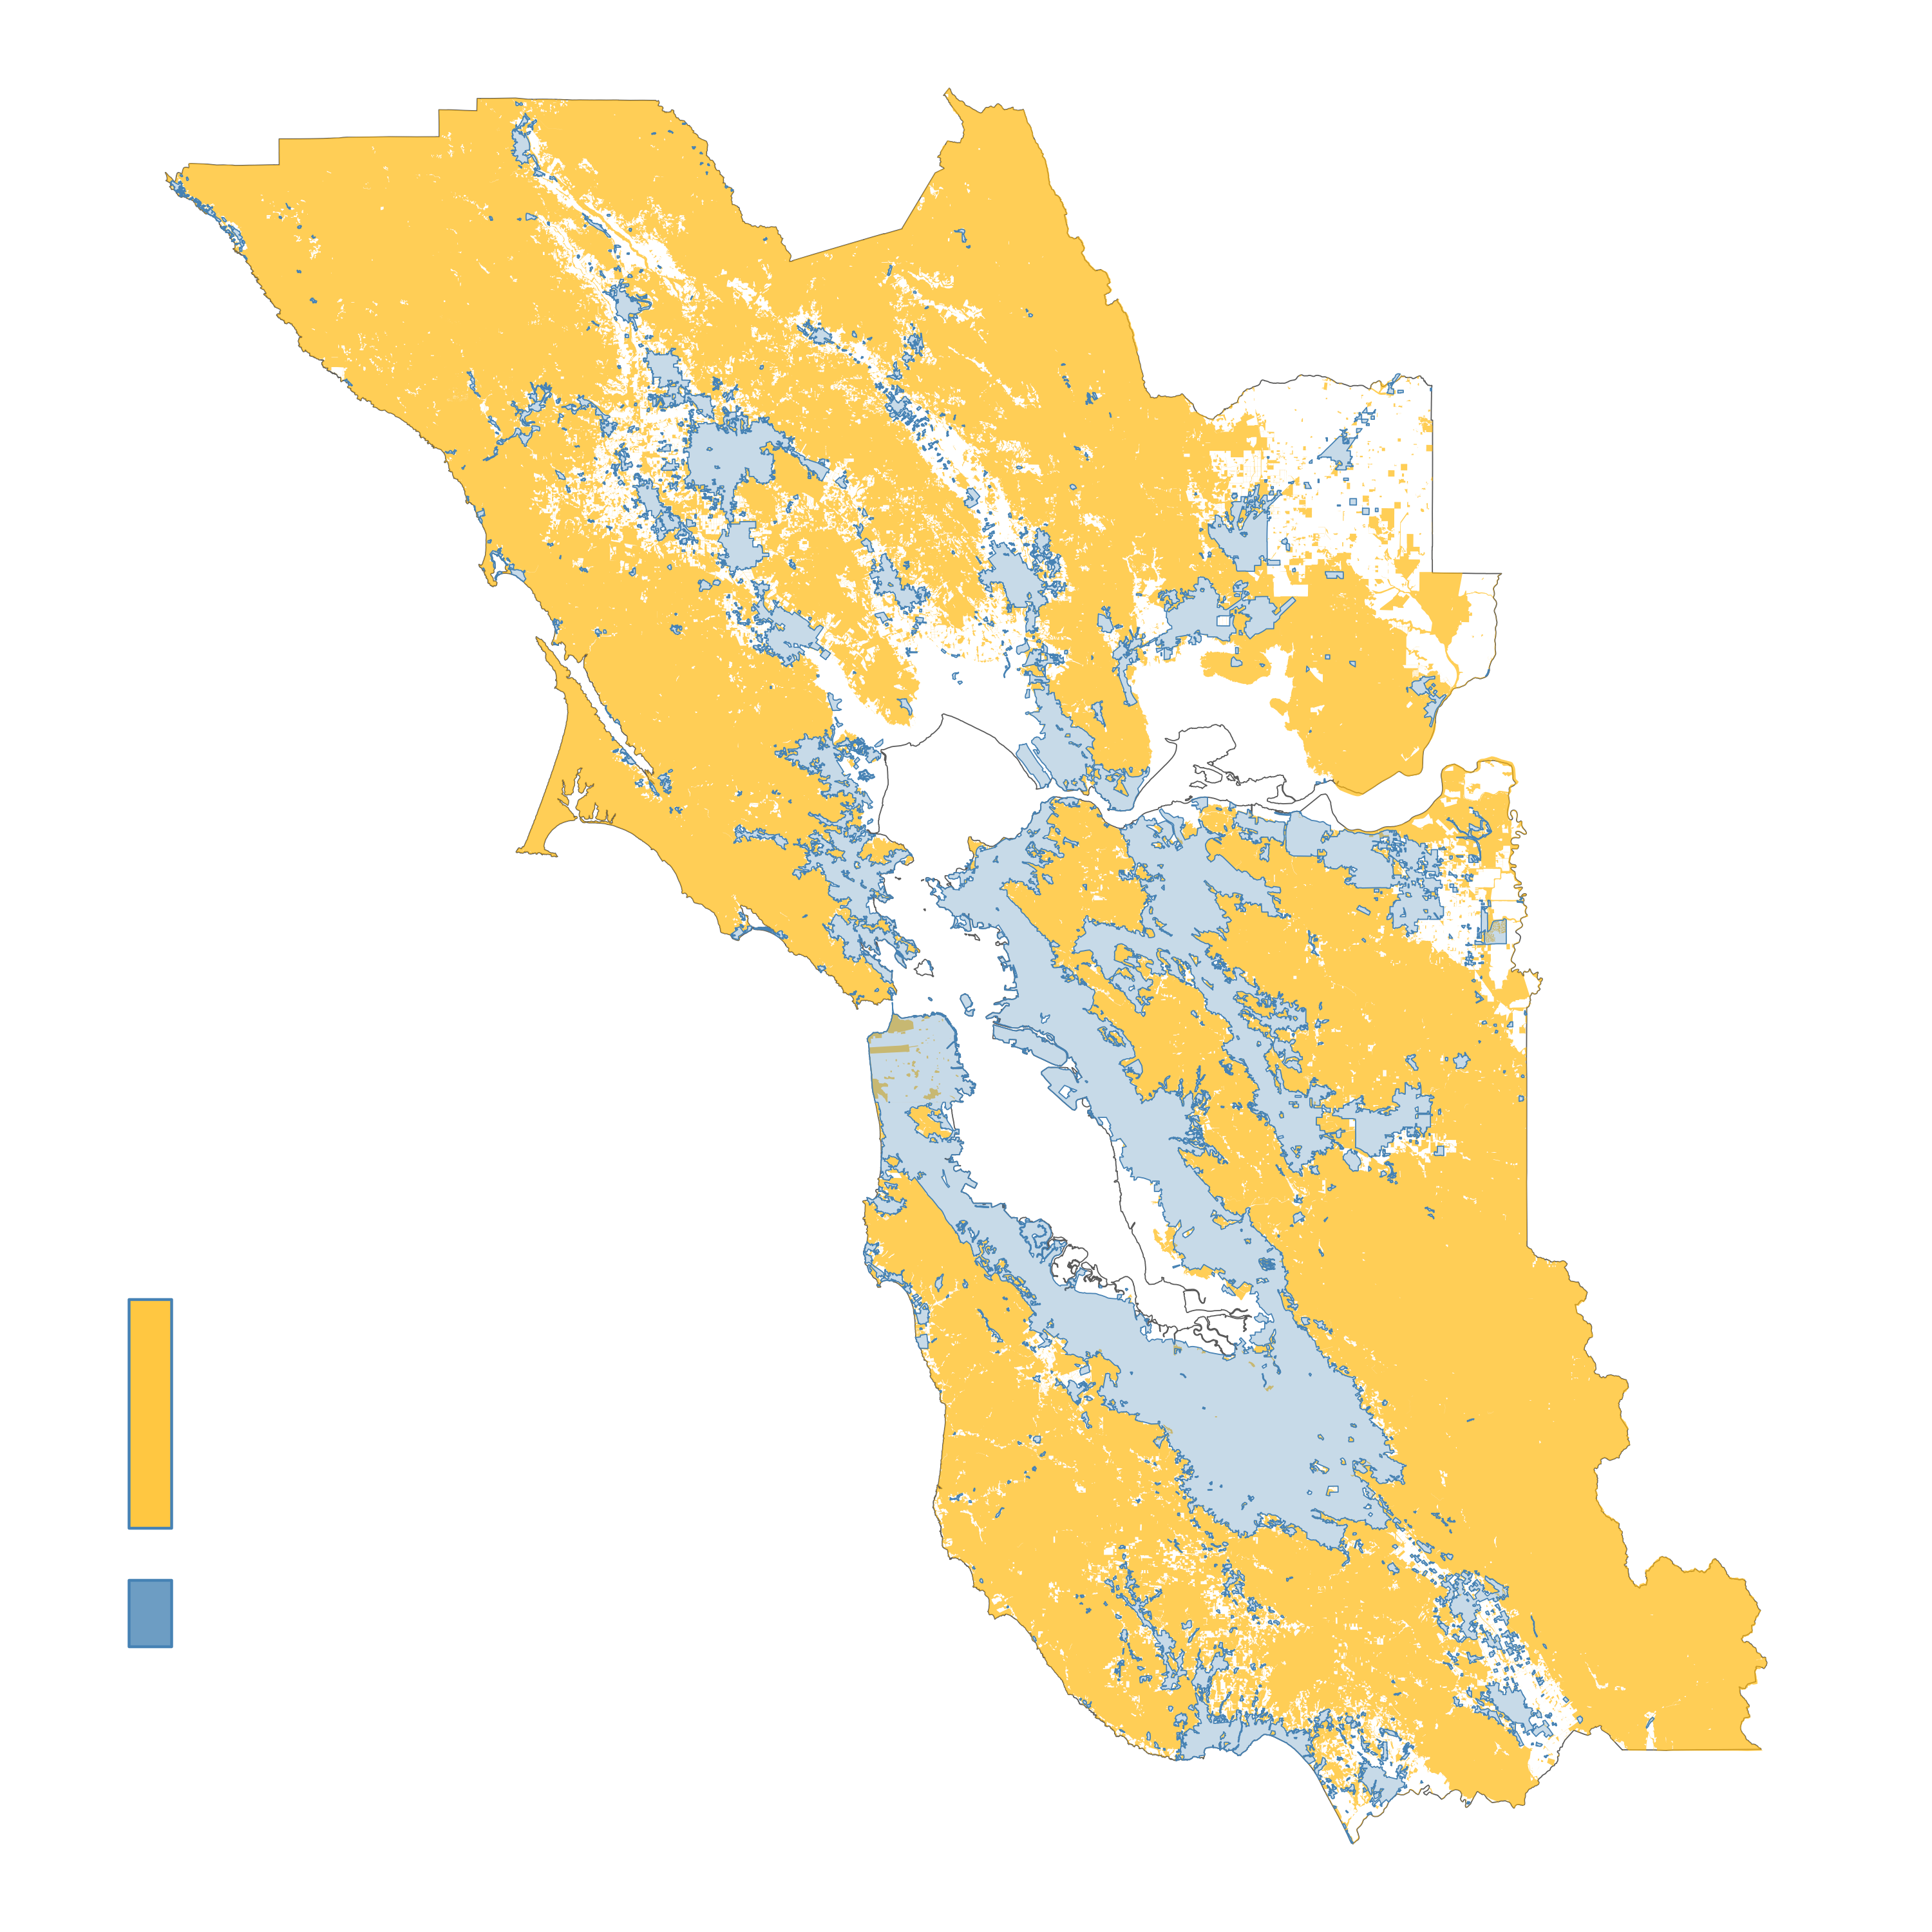
\includegraphics[width=.3\textwidth]{img/urbancln.png}
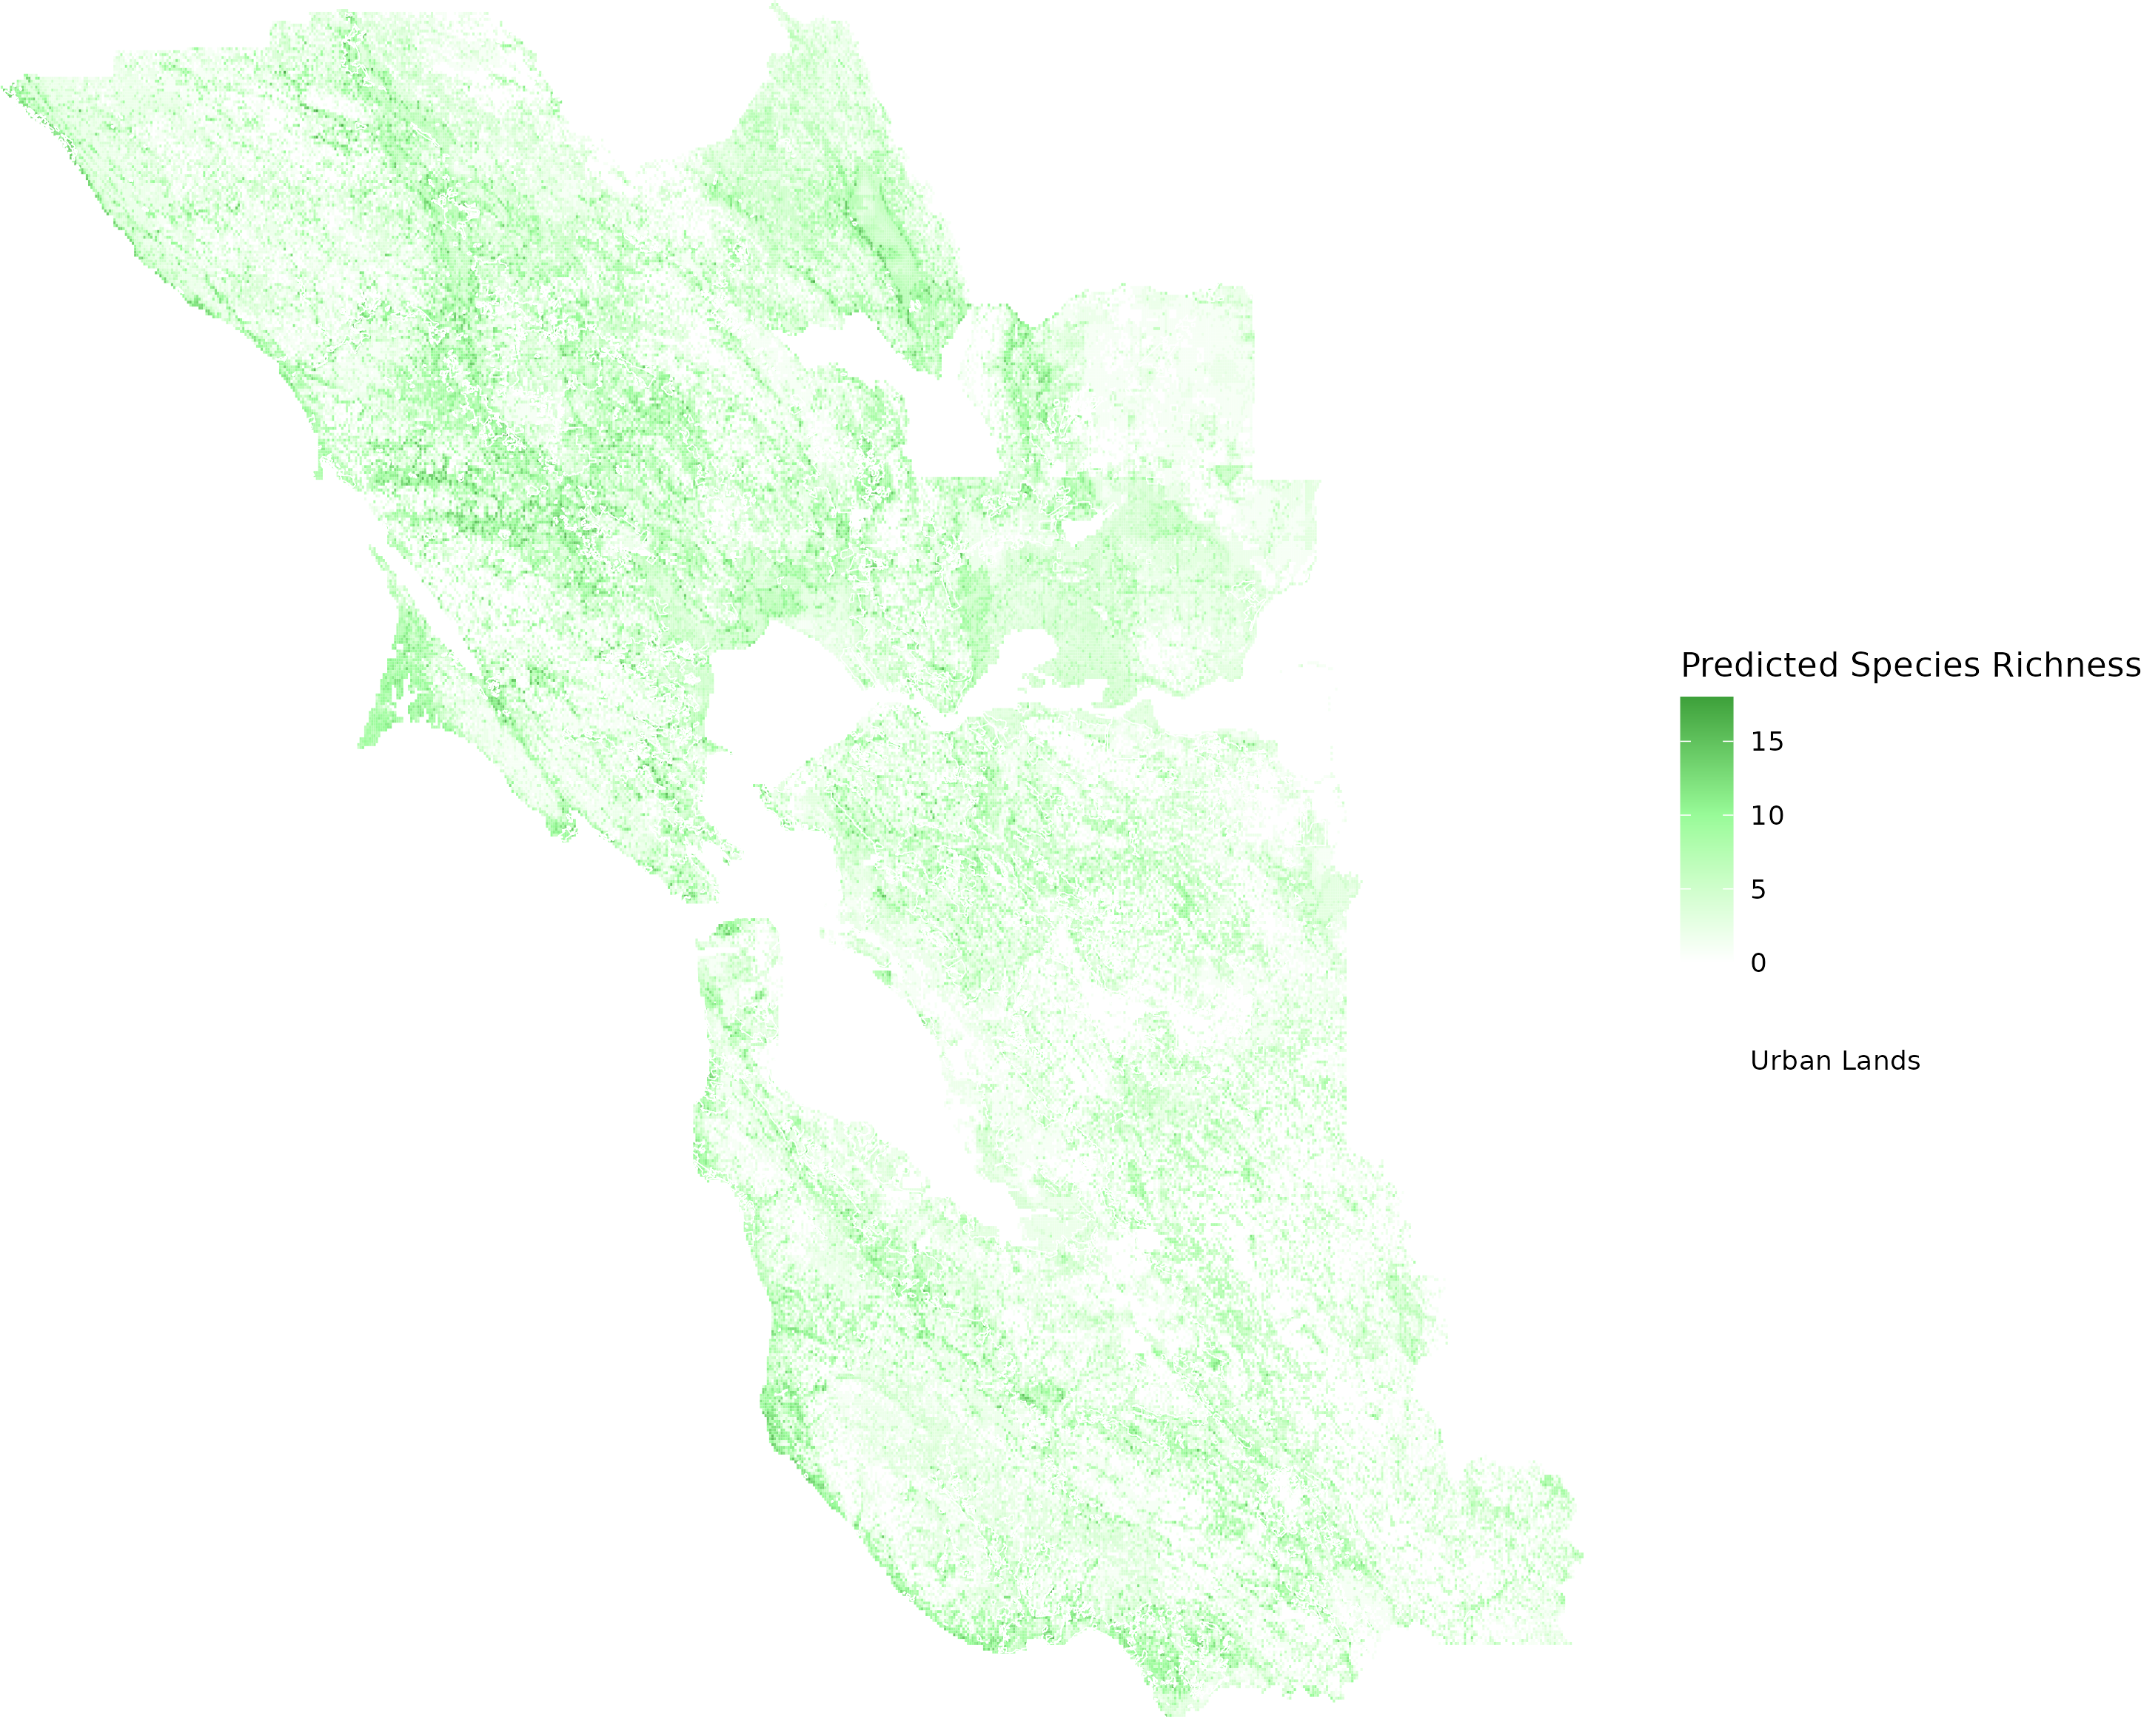
\includegraphics[width=.7\textwidth]{img/species_richness.png}
% \\\textbf{Emphasize} the important words.
\vfill
}{
%%%% Bottom space

%% QR code
\qrcode{img/qr-code}{img/smartphoneWhite}{
\textbf{Take a picture} to
\\access the interactive report
\\we sent to community collaborators
}
% Smartphone icon
% Author: Freepik
% Retrieved from: https://www.flaticon.com/free-icon/smartphone_65680

}

}{
%%%%%%%% LEFT COLUMN

\title{Using iNaturalist to evaluate the contribution of urban landscapes to regional conservation goals}
\author{Avery Hill$^1$, Tom Robinson$^2$, Rebecca Johnson$^1$, Alison Young$^1$}

\institution{$^1$California Academy of Sciences}
\institution{$^2$Together Bay Area}

\section{Introduction}

\vspace{-2cm}
\begin{itemize}
\item Regional \textbf{conservation} organizations in the San Francisco Bay Area have \textbf{not yet recognized} the extent to which \textbf{urban lands} provide habitat for target conservation species.
\item The biodiversity community science platform, \textbf{iNaturalist}, demonstrates that many \textbf{target species} are \textbf{frequently observed} in urban landscapes.
\item \textbf{Species distribution modeling} (SDM) is a powerful tool for evaluating the habitat of target species and mapping available habitat across urban areas.
\end{itemize}

\section{Materials \& Methods}
% We trained SDMs for X species using regional iNaturalist observations and X environmental variables.
% \vspace{1cm}
\def\iconspace{3mm}
\vspace{-14mm}
\\\faMapO   \hspace{1cm} 10 San Francisco Bay Area counties
\vspace{\iconspace}
\\\faClockO \hspace{1cm} 1999 - 2023
\vspace{\iconspace}
\\\faMapMarker \hspace{1cm} 53,000 observations across 20 species
\vspace{\iconspace}
\\\faSunO \hspace{1cm} 18 environmental variables at 10m
\vspace{\iconspace}
\\\faConnectdevelop \hspace{1cm} Maxent SDM, 5-fold cross validation
\vspace{\iconspace}
\\\faCode \hspace{1cm} R v4.2.2, \textit{SDMTune}, \textit{blockCV}, \textit{terra}, 
\\ \hspace*{2.1cm} \textit{tidyverse}, \textit{CoordinateCleaner}, \textit{sf}
\begin{center}

% \includegraphics[width=\textwidth]{img/tikzexample1}
\end{center}




}{
%%%%%%%% RIGHT COLUMN
\section{Results}

Species Table

\includegraphics[width=\textwidth]{img/species_table.png}
% \begin{longtable}{l|rrr}
\toprule
\multicolumn{1}{l}{} & Presence Points & AUC & TSS \\ 
\midrule
Aneides lugubris & 1815 & 0.82 & 0.48 \\ 
Aphelocoma californica & 5902 & 0.79 & 0.42 \\ 
Callipepla californica & 2952 & 0.86 & 0.56 \\ 
Canis latrans & 3354 & 0.86 & 0.54 \\ 
Chlorogalum pomeridianum & 3873 & 0.85 & 0.52 \\ 
Danaus plexippus & 3904 & 0.90 & 0.64 \\ 
Elgaria coerulea & 506 & 0.93 & 0.71 \\ 
Elgaria multicarinata & 1809 & 0.79 & 0.43 \\ 
Helminthoglypta nickliniana & 155 & 0.95 & 0.77 \\ 
Juglans hindsii & 81 & 0.94 & 0.73 \\ 
Lontra canadensis & 602 & 0.98 & 0.85 \\ 
Melanerpes formicivorus & 4116 & 0.86 & 0.56 \\ 
Nycticorax nycticorax & 3346 & 0.96 & 0.78 \\ 
Sciurus griseus & 1375 & 0.92 & 0.68 \\ 
Sialia mexicana & 5075 & 0.84 & 0.51 \\ 
Thamnophis elegans & 308 & 0.91 & 0.66 \\ 
Thamnophis sirtalis & 38 & 0.97 & 0.86 \\ 
Zonotrichia leucophrys & 5198 & 0.89 & 0.63 \\ 
\bottomrule
\end{longtable}


Predictor Table


\vfill

%% Institution logo
\begin{center}


\includegraphics[width=.8\textwidth]{img/combined_logo.eps}\\
% \end{right}
\end{center}
}
\end{document}
